\documentclass[a4paper,]{article}
\usepackage{libertine}
\usepackage[T1]{fontenc}
\usepackage[utf8]{inputenc}
\usepackage{geometry}
\geometry{%
	left   = 2cm,
	right  = 2cm,
	top    = 2cm,
	bottom = 2cm
}
\usepackage{setspace}
\setstretch{1}

\usepackage[nolist]{acronym}
\usepackage{commath}
\usepackage{verbatim}
\usepackage{listings}
\usepackage{enumitem}
\usepackage{graphicx,color,psfrag}
\usepackage{subfigure}
\usepackage{svg}
\usepackage{svg-extract}
\usepackage{todonotes}
\usepackage[acronym,nonumberlist,nowarn,style=long]{glossaries}

\newacronym{acr:FPGA}{FPGA}{field programmable gate array}
\newacronym{acr:IP}{IP}{intellectual property}
\newacronym{acr:ILA}{ILA}{integrated logic analyzer}
\newacronym{acr:CNN}{CNN}{convolutional neural network}
\newacronym{acr:DMA}{DMA}{direct memory access}
\newacronym{acr:PS}{PS}{processing system}
\newacronym{acr:PL}{PL}{programmable logic}
\newacronym{acr:BRAM}{BRAM}{block-RAM}

\begin{document}
\begin{titlepage}
	
	\begin{flushright}
		
		% Update this with your team number]
		
		% Update this with your matriculation number, first name, second name
		\Large 
		Yellow Of The Egg\\
		\large
		Lukas Baischer	\\
		Add your names .. \\
		
	\end{flushright}
	
	\vspace{5em}
	
	\begin{center}
		{\Large SoC Design Laboratoy}\\[1em]
		{\large 384.157, Winter Term 2019} \\[5em]

		
		{\Huge MNIST-FPGA\\[.5em]
		\huge Specification}\\[10em]
	\end{center}
	
	
	%	\begin{abstract}
	%
	%		Enter the abstract of your report here. An abstract summarizes your
	%		entire work (i.e., problem statement, motivation, methodology, key
	%		findings). It is a good strategy to write a first version of the abstract
	%		when you start to work on your report. This gives you a good guideline
	%		what to	put and what not to put into the report. Ideally, you re-write
	%		the abstract once you finished your report, because only at this point
	%		you have all the information available to create a good abstract.
	%
	%	\end{abstract}
	
\end{titlepage}


\begin{acronym}
	\acro{FPGA}{Field Programmable Gate Array}
	\acro{FIFO}{First In, First Out}
	\acro{CNN}{Convolutional Neural Network}
\end{acronym}
\section{Introduction}


\section{Concept}

\subsection{Neural Network}

For the neural network we base the architecture of our network on the well known \emph{LeNet} architecture from \cite{LeCun:1998aa} is chosen due to its simplicity and ease to implement. Additionally the performance is improved by using modern, established techniques like batch normalization \cite{Ioffe:2015aa} and dropout \cite{Srivastava:2014aa} layers. 
The training of network is done using PyTorch \cite{Paszke:2019aa} on a regular PC and the trained network parameters are then used to create a hardware VHDL model of the network. An overview of the structure can be seen in Figure~\ref{fig:network-concept}. For verification all neural network operations are checked in separate programmed programs for correctness. See the Section~\ref{subsec:nntraining} for details how the network is implemented in Software.
An excellent overview in deep learning can be found in \cite{Schmidhuber:2015aa}.
To train and test the network we chose the MNIST dataset \cite{LeCun:1998ab}. It consists of 50.000 training images and 10.000 test images of handwritten digits, where each is 28-by-28 pixel.


\begin{figure}[htbp]
	\noindent\resizebox{\textwidth}{!}{
	\begin{tikzpicture}
		%\draw[use as bounding box, transparent] (-1.8,-1.8) rectangle (17.2, 3.2);

		% Define the macro.
		% 1st argument: Height and width of the layer rectangle slice.
		% 2nd argument: Depth of the layer slice
		% 3rd argument: X Offset --> use it to offset layers from previously drawn layers.
		% 4th argument: Options for filldraw.
		% 5th argument: Text to be placed below this layer.
		% 6th argument: Y Offset --> Use it when an output needs to be fed to multiple layers that are on the same X offset.

		\newcommand{\networkLayer}[6]{
			\def\a{#1} % Used to distinguish input resolution for current layer.
			\def\b{0.02}
			\def\c{#2} % Width of the cube to distinguish number of input channels for current layer.
			\def\t{#3} % X offset for current layer.
			\def\d{#4} % Y offset for current layer.

			% Draw the layer body.
			\draw[line width=0.3mm](\c+\t,0,\d) -- (\c+\t,\a,\d) -- (\t,\a,\d);                                                      % back plane
			\draw[line width=0.3mm](\t,0,\a+\d) -- (\c+\t,0,\a+\d) node[midway,below] {#6} -- (\c+\t,\a,\a+\d) -- (\t,\a,\a+\d) -- (\t,0,\a+\d); % front plane
			\draw[line width=0.3mm](\c+\t,0,\d) -- (\c+\t,0,\a+\d);
			\draw[line width=0.3mm](\c+\t,\a,\d) -- (\c+\t,\a,\a+\d);
			\draw[line width=0.3mm](\t,\a,\d) -- (\t,\a,\a+\d);

			% Recolor visible surfaces
			\filldraw[#5] (\t+\b,\b,\a+\d) -- (\c+\t-\b,\b,\a+\d) -- (\c+\t-\b,\a-\b,\a+\d) -- (\t+\b,\a-\b,\a+\d) -- (\t+\b,\b,\a+\d); % front plane
			\filldraw[#5] (\t+\b,\a,\a-\b+\d) -- (\c+\t-\b,\a,\a-\b+\d) -- (\c+\t-\b,\a,\b+\d) -- (\t+\b,\a,\b+\d);

			% Colored slice.
			\ifthenelse {\equal{#5} {}}
			{} % Do not draw colored slice if #4 is blank.
			{\filldraw[#5] (\c+\t,\b,\a-\b+\d) -- (\c+\t,\b,\b+\d) -- (\c+\t,\a-\b,\b+\d) -- (\c+\t,\a-\b,\a-\b+\d);} % Else, draw a colored slice.
		}

		% INPUT
		\node[] (input image) at (-3.75,0.5) {
\includegraphics[height=30mm]{img/mnist/mnist_input_5_28}};
		\networkLayer{3.0}{0.03}{-0.5}{0.0}{color=gray!80}{}

		% ENCODER
		\networkLayer{3.0}{0.1}{0.0}{0.0}{color=white}{conv}    % S1
		%\networkLayer{3.0}{0.1}{0.2}{0.0}{color=white}{}        % S2
		\networkLayer{2.5}{0.2}{0.6}{0.0}{color=white}{conv}    % S1
		\networkLayer{2.5}{0.2}{0.9}{0.0}{color=white}{}        % S2
		\networkLayer{2.0}{0.4}{1.3}{0.0}{color=white}{conv}    % S1
		\networkLayer{2.0}{0.4}{1.8}{0.0}{color=white}{}        % S2
		\networkLayer{1.5}{0.8}{2.3}{0.0}{color=white}{conv}    % S1
		\networkLayer{1.5}{0.8}{3.2}{0.0}{color=white}{}        % S2
		\networkLayer{1.0}{1.5}{4.1}{0.0}{color=white}{conv}    % S1
		\networkLayer{1.0}{1.5}{5.7}{0.0}{color=white}{}        % S2

		% DECODER
%		\networkLayer{1.0}{1.5}{7.7} {0.0}{color=white}{deconv} % S1
%		\networkLayer{1.0}{1.5}{9.3} {0.0}{color=white}{}       % S2
%		\networkLayer{1.5}{0.8}{11.2}{0.0}{color=white}{deconv} % S1
%		\networkLayer{1.5}{0.8}{12.1}{0.0}{color=white}{}       % S2
%		\networkLayer{2.0}{0.4}{13.3}{0.0}{color=white}{}       % S1
%		\networkLayer{2.0}{0.4}{13.8}{0.0}{color=white}{}       % S2
%		\networkLayer{2.5}{0.2}{14.8}{0.0}{color=white}{}       % S1
%		\networkLayer{2.5}{0.2}{15.1}{0.0}{color=white}{}       % S2
%		\networkLayer{3.0}{0.1}{15.8}{0.0}{color=white}{}       % S1
%		\networkLayer{3.0}{0.1}{16}  {0.0}{color=white}{}       % S2

		% OUTPUT
%		\networkLayer{3.0}{0.05}{17}{0.0}{color=red!40}{}          % Pixelwise segmentation with classes.
%		\node[] (output image) at (18,0.5) {\includegraphics[height=30mm]{vermeer.jpg}};
%

	\end{tikzpicture}
	}
	\caption{Example CNN.}
	\label{fig:network-concept}
\end{figure}

\subsection{Hardware Concept}
\begin{figure}[h]
	\centering
	\includesvg[width=\textwidth]{img/inkscape/NN-concept.svg}
	\caption[Top-Level concept.]{Top-Level concept}
	\label{FIG:concept}
\end{figure}
\todo{Maybe add an additional Input Layer which is responsible to communicate with the DMA and converts the data from 32 bit to 8 bit and sends it to the memory controller}
\noindent
Figure \ref{FIG:concept} shows the Concept of implementing an FPGA-based hardware accelerator for handwritten digit recognition. It shows that the main components of the concepts are a Zedboard in combination with a remote PC or server. The handwritten digit recognition is performed by the Zedboard while the remote PC is used for training the network, for sending the image data to the Zedboard and for receiving the computed results.  The Zedboard includes a Zynq-7000 FPGA and provides various interfaces. \\
The neural network is implemented in the programmable logic part of the Zynq-7000. It is pre-trained using the remote PC, therefore only the inference of the neural network is implemented in hardware. \\
In order to train the network with the same bit resolution as implemented in the hardware, a software counterpart of the hardware is implemented in a PC using python. 
Based on the weights calculated by the python script a bitstream for the hardware is generated. This brings the benefit that for the convolutional layer constant multiplier can be used, since the weights of convolutional layer kernels are constant. For the dense layer it is not possible to implement the weights in a constant multiplier because in a dense layer each connection of a neuron requires a different weight, which would result in a huge amount of required constant multipliers. Therefore the weights for the dense layer have to be stored in a ROM inside the FPGA.   \\


\section{Software}

\subsection{Host software}

The remote software is either implemented on a PC or on a server. It is used for performing the training of the network and for generating a FPGA-bitstream based on the computed weights. Additionally the remote software is used to send the image data to the Zedboard and receive the results of the network for each image. 

Therefore the Host software can be separated in two parts:
\begin{itemize}
	\item Trainings software
	\item Communication software
\end{itemize} 

Requirements of the Trainings Software:
\begin{itemize} 
	\item Training of the network considering bit resolution of implemented hardware
	\item Create VHDL code based on the network hyper-parameter and on the computed weights
	\item Create a bitstream with the generated VHDL code
\end{itemize}

Requirements of the Trainings Software:
\begin{itemize}
	\item Sends image data to Zedboard
	\item Receives results from Zedboard
	\item Create a figure of accuracy and performance   
	\item Optional: Send bitstream to hardware which updates the bitstream 
\end{itemize}

\subsubsection{Interface to Zedboard} \label{subsec:InterfaceRemoteZed}
Ethernet is used for the communication of the remote host system and the embedded Linux which is running on the Zedboard. 
The embedded Linux distribution running on the board should automatically receive an IP address when connected to a network. When in doubt the address can be found out with the \texttt{ifconfig} command. 
The software has a client-server model with the embedded system acting as a server and the host as a client. Once running, the server software is listening for new outside connections. Different types of data need to be transmitted:

\begin{itemize}
	\item The 28x28 input images showing digits between 0 and 9 is transferred from host to Zedboard.
	\item The probability of resulting numbers between 0 and 9 is transmitted from Zedboard to host.
	\item control and status signals in both directions 
	\item Optional: Bitstream file for dynamically update the bitstream at the Zedboard
\end{itemize}

\subsubsection{Notes}
On Windows host systems, \emph{Network Discovery} needs to be enabled and in some cases a Firewall exception for the used ports needs to be set for a connection to be established. \\
\subsection{ARM Top-Level Software}
The ARM top-level software receives the image data from a remote device and sends the results back to this device. Control of the hardware.

\subsubsection{Requirements}
\todo{Add more information and specify the requirements}
Requirements of the ARM Top-Level Software:
\begin{itemize} 
	\item Receive image data
	\item Also use image data set already stored on device
	\item send results to remote PC
	\item Send and receive control signals from remote PC
	\item Send image data to driver user layer and receive results from driver user layer
	\item Send and receive status and control signals to driver user layer
	\item Run at start-up 
\end{itemize}

\subsubsection{Dynamic Updating of the Bitstream}

Optional feature: Update Bitstream file using \texttt{/dev/xdevcfg}.

Update: For newer versions it looks like \texttt{/dev/xdevcfg} doesn't exist anymore. The problem is discussed here \footnote{\url{https://forum.digilentinc.com/topic/18194-dynamically-load-bitstream-on-petalinux/}} and a potential solution can be found here. \footnote{\url{https://github.com/Digilent/zynq-dynamic-tools}}

\subsubsection{Interface to remote PC}
See Section \ref{subsec:InterfaceRemoteZed}.  
\subsubsection{Interface to kernel layer}
Python wrapper are used for the interface between the top level software which is programmed in python and the hardware drivers which are programmed in C. For usability a high level interface to the underlying C wrapper is made. 
This header interface can then be wrapped to multiple target languages using \cite{Swig2020}. In our case this was done for Python.

\subsubsection{File Tree of ARM Top-Level software} \label{SEC:ARM-TOP-SW-FILE-TREE} \todo{Update this section. Do we still use the C code or do we plan to implement everything in python?}
\begin{figure}[h] 
	\centering
	{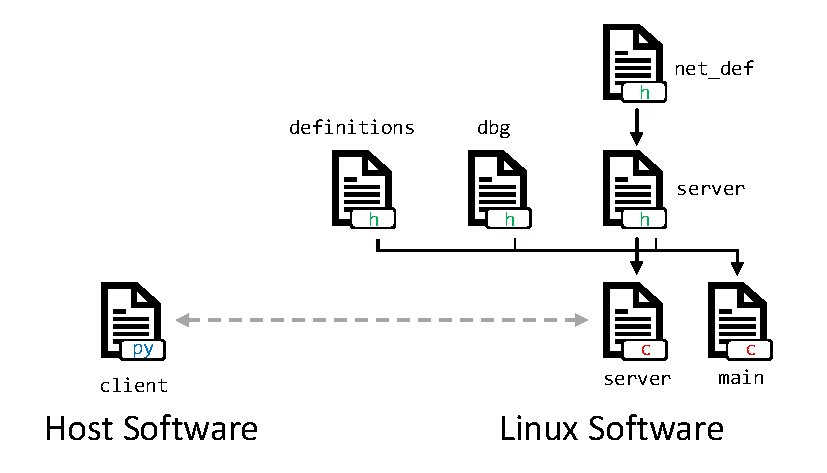
\includegraphics[scale=0.75]{img/software.pdf}} 
	\caption{File tree for the software}
\end{figure} 
\begin{itemize}
	\item \verb|net_def.h| Contains definitions for networking, e.g. ports used.
	\item \verb|dbg.h| Contains debugging macros for logging and error handling.
	\item \verb|definitions.h| Contains information about the neural network, e.g. the number and type of \ac{CNN} stages, layers in the fully connected network, input size and so on.
	\item \verb|server.{c,h}| Handles the connection with the host software.
	\item \verb|main.c| Contains the \verb|main()| function with the main program loop that transmits and manages data to the hardware and from the host system.
	\item \verb|client.py| Handles the connection with the client software.
\end{itemize}

\subsection{User Layer Driver Software}
The user layer driver software implements an interface between the ARM Top-Level software and the driver for the programmable logic. It is implemented in C. It is supposed to handle the entire communication with the driver so that the hardware is only abstractly visible for the ARM Top-Level software.\\
For example the ARM top-level software sees the network as a class in python which has a methode\_load\_new\_image data with a numpy array as input and a finish signal as a output. This method should call the user layer driver software which handles the communication between user space and kernel space. In a similar way each IP should be a class in python. \\
Requirements of the User Layer Driver Software:
\begin{itemize} 
	\item Communication with the kernel space drivers 
	\item Use python wrapper to communicate with ARM Top-Level software
	\item Easy to use interface from Top-Level 
	\item No knowledge of the hardware should be necessary to use the interface
	\item Data encapsulation to avoid the Top-Level Software from corrupting the memory 
\end{itemize}

\subsubsection{File Tree of User Layer Driver Software} \todo{Would be nice if we have something similar as in \ref{SEC:ARM-TOP-SW-FILE-TREE}}



\section{Hardware}
\subsection{Memory Controller}
The task of the memory controller is to provide valid data for the NN-layers. It communicates with the Block-Ram. The memory controller is responsible for ensuring that the next layer has valid data at all times. The second task of the memory controller is to save the data of the previous data in a free memory address in the Block-RAM. 
\todo{Is it better to have the shiftregister, we discussed last time in the memory controller, because in this case the layer don't have to know anything about the data it gets}

\subsubsection{Interfaces}
\begin{itemize}
	\item S\_LAYER: interface to previous layer
	\item M\_LAYER: interface to next layer 
	\item AXI\_lite: interface to AXI lite bus, is used to read BRAM data directly from processor (slow)
\end{itemize}
\begin{tabular}{|l|l|l|l|l|}
	
	signal & direction & type & width & description\\
	
\end{tabular}

\begin{itemize}
	\item M\_LAYER: interface to next layer
\end{itemize}
\begin{tabular}{|l|l|l|l|l|}
	
	signal & direction & type & width & description\\
	
\end{tabular}

\begin{itemize}
	\item BRAM\_PORTA: write interface to BRAM
\end{itemize}
\begin{tabular}{|l|l|l|l|l|}
	
	signal & direction & type & width & description\\
	
\end{tabular}

\begin{itemize}
	\item BRAM\_PORTB: read interface to BRAM
\end{itemize}
\begin{tabular}{|l|l|l|l|l|}
	
	signal & direction & type & width & description\\
	
\end{tabular}

\subsubsection{Parameter}
\begin{itemize}
	\item PREVIOUS\_LAYER\_TYPE boolean: {TRUE: conv2d, FALSE: dense} % maybe some additional -> integer type
	\item PREVIOUS\_LAYER\_WIDTH integer: {Row length of input matrix} \todo{use extra parameter for dense or simply use width or height, discuss!}
	\item PREVIOUS\_LAYER\_HEIGTH integer: {Column length of input matrix}
	\item PREVIOUS\_LAYER\_CHANNEL integer: {Row length of input matrix}
	\item NEXT\_LAYER\_TYPE boolean: {TRUE: conv2d, FALSE: dense} % maybe some additional -> integer type
	\item NEXT\_LAYER\_WIDTH integer: {Row length of input matrix} \todo{use extra parameter for dense or simply use width or height, discuss!}
	\item NEXT\_LAYER\_HEIGTH integer: {Column length of input matrix}
	\item NEXT\_LAYER\_CHANNEL integer: {Row length of input matrix}
\end{itemize}

\subsection{AXI lite interface}
It is used to read the BRAM data directly from the processor. This can be used for debug purposes. \\
Each memory controller gets an unique address via generics. 
One 32 bit register of the AXI lite bus is used for all memory controller. 
If the processor writes all 0 to the register, debugging mode is deactivated. 
Therefore the memory controller address start with 1 and not with 0.
the 32 bit are separated as follows: \\
\begin{itemize}
	\item 23 downto 0: BRAM address
	\item 27 downto 24: 32 bit vector address 
	\item 31 downto 28 : Memory controller address 
\end{itemize}  
BRAM address: address of the block ram \\
32 bit vector address: If the width of one BRAM register is higher than 32 bit, the 32 bit vector address can be used to select the required part of the vector. \\
Memory controller address: address of the memory controller used in the network starting with 1. If the address of the memory controller is selected debug mode is active. \\

 
\subsection{conv2d}

\begin{figure}[h]
	\centering
	\includesvg[width=0.7\textwidth]{img/inkscape/conv2d.svg}
	\caption[Conv2d block diagram.]{Conv2d block diagram. For each output channel a conv\_channel module is used. $k$ indicates the number of output channels.}
	\label{FIG:conv2d}
\end{figure}
Figure \ref{FIG:conv2d} shows the block diagram of a conv2d module. It uses $k$ conv\_channel modules to realise $k$ output channels. 
All conv\_channel modules get the same input vector $X_{c_i}$. All conv\_channel modules
and the two conv2d modules are automatically generated by a Python script.
\subsubsection{Interface}
\begin{itemize}
	\item Input interface connected to shift register, which consists of a $n \cdot 3 \times 3$ vector of values of length BIT\_WIDTH\_IN, in which $n$ is the number of input channels.
	\item Output interface connected to the pooling layer, which is a vector of $m$ values of length BIT\_WIDTH\_OUT, in which $m$ is the number of output channels.
\end{itemize}
Both input and output interfaces have ready, last and valid signals to control the flow of data.
\subsubsection{Parameter}
\begin{itemize}
 	\item BIT\_WIDTH\_IN : integer
 	\item BIT\_WIDTH\_OUT : integer
 	\item INPUT\_CHANNELS: integer
 	\item OUTPUT\_CHANNELS: integer
\end{itemize}
\subsection{conv\_channel}

\begin{figure}[h]
	\centering
	\includesvg[width=0.7\textwidth]{img/inkscape/conv-channel.svg}
	\caption[conv\_channel block diagram.]{conv\_channel block diagram. For each input channel a kernel\_3x3 module is used. $n$ indicates the number of input channels.}
	\label{FIG:conv-channel}
\end{figure}
Figure \ref{FIG:conv-channel} shows the block diagram of a conv\_channel module. It uses $n$ kernel\_3x3 modules to realise $n$ input channels. 
All kernel\_3x3 modules get a different input vector $X_{c_{i1}}$ to $X_{c_{in}}$ which are $3 \times 3$ input matrices.   
\subsubsection{Interface}
\todo{define input output interface}

\subsubsection{Parameter}
\begin{itemize}
 	\item INPUT\_CHANNEL\_NUMBER : integer
 	\item OUTPUT\_CHANNEL\_NUMBER : integer
 	\item MATRIX\_WIDTH: integer
 	\item MATRIX\_HEIGTH: integer
\end{itemize}
\subsection{kernel-3x3}
This modules performs a multiplication of 9 values of length BIT\_WIDTH\_IN with their respective weights which are defined in an
array that can be set with a generic. The multiplication results are then added up, after which a ReLu step is performed where outputs
above 255 are clipped to 255 and outputs below 0 are clipped to 0.
\subsubsection{Interface}
\begin{itemize}
	\item Input interface, a vector of 9 values of length BIT\_WIDTH\_IN.
	\item Output interface, same as conv\_channel.
\end{itemize}
\subsubsection{Parameter}
\begin{itemize}
	\item BIT\_WIDTH\_IN: integer
	\item BIT\_WIDTH\_OUT: integer
	\item WEIGHT: array of 9 integers
	\item WEIGHT\_WIDTH: integer
\end{itemize}
\subsection{Dense Layer}

\subsubsection{Operation}
\begin{figure}[h]
	\centering
	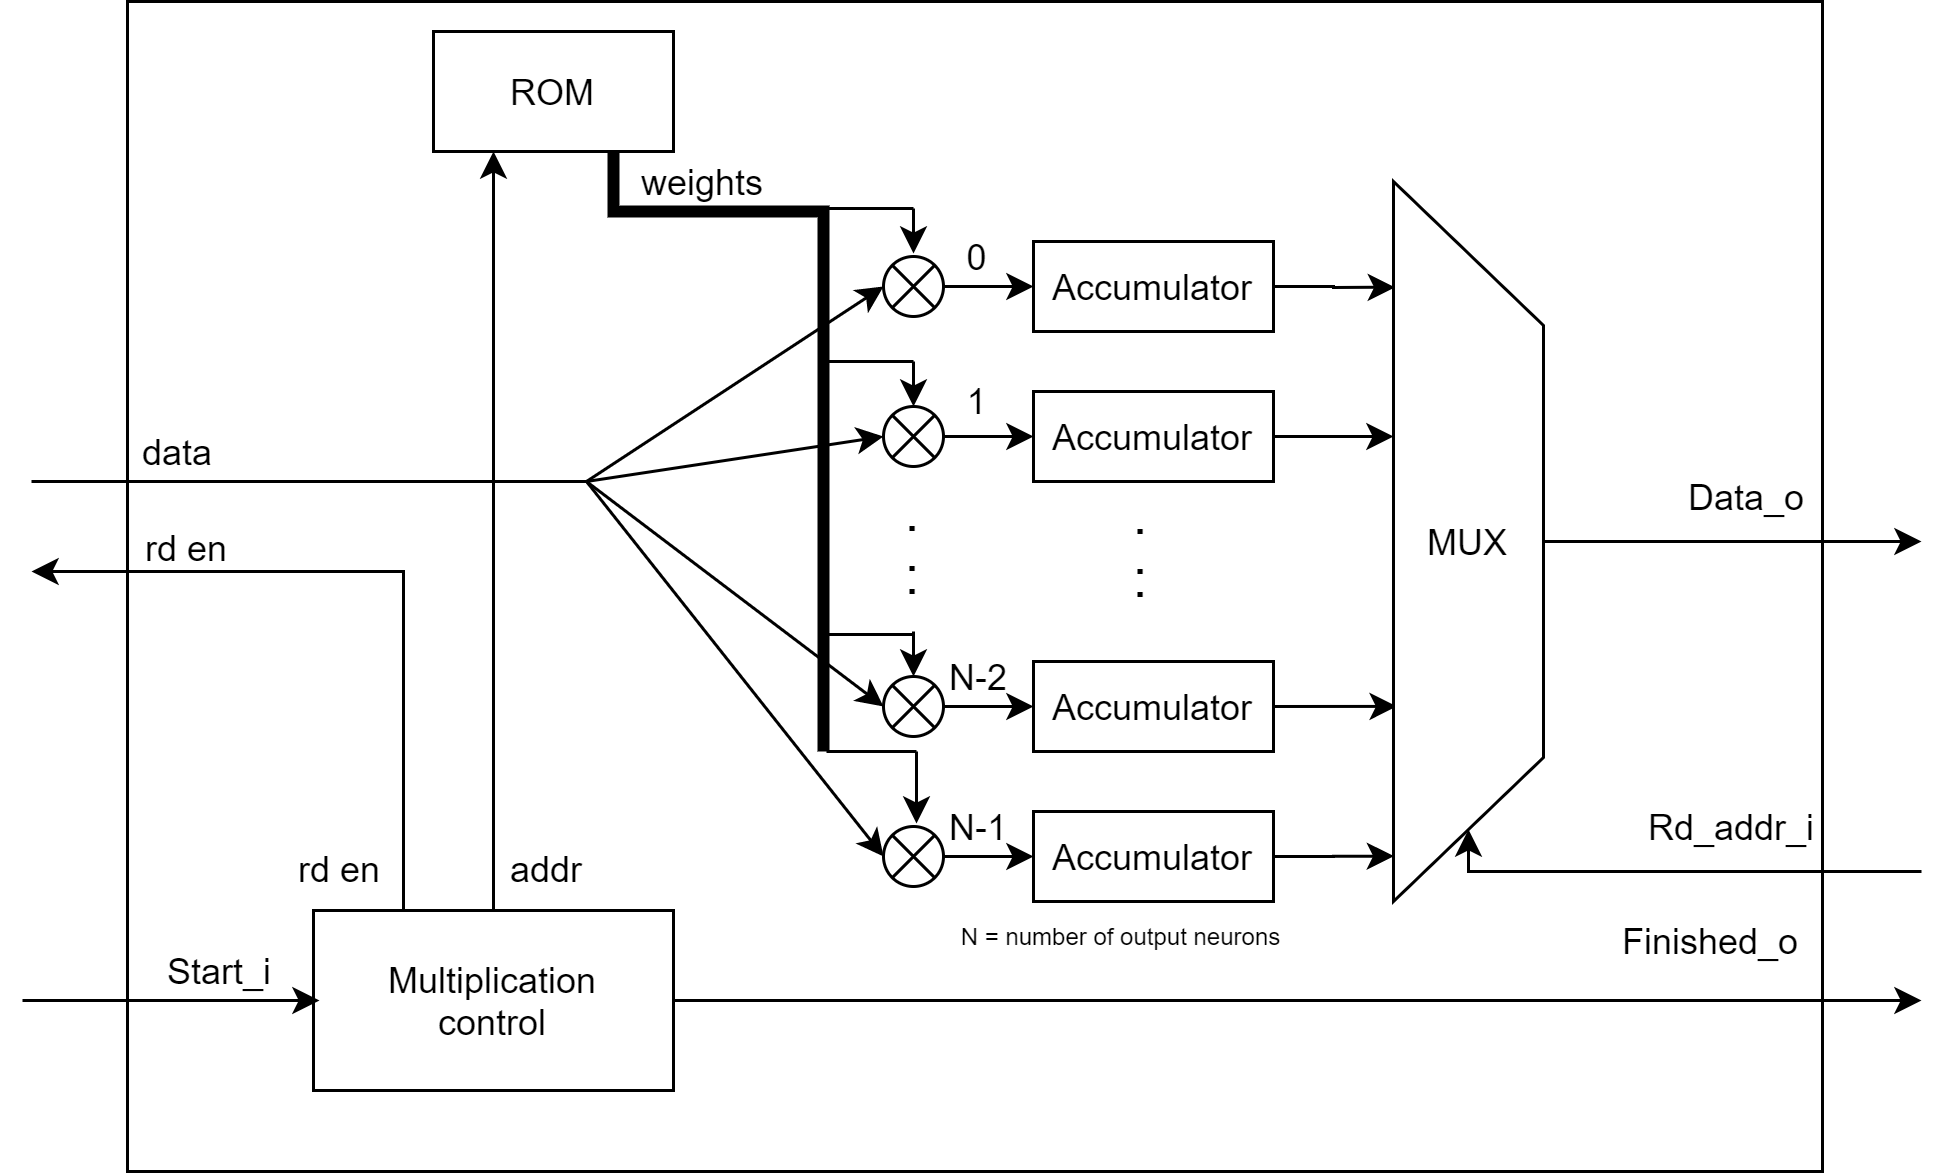
\includegraphics[width=1\textwidth]{img/blockDiagramDense.png}
	\caption[Dense layer diagram]{Dense layer diagram.}
	\label{FIG:denseLayerBlockDiagram}
\end{figure}


(Schematic is on figure \ref{FIG:denseLayerBlockDiagram}.)
This block contains a finite state machine. When the Start\_i input port goes high, input neurons are read from an external FIFO one by one. Each of the input neurons is multiplied by appropriate weight for each of the output neurons. These product are then fed to accumulators, which make a sum of all products of all neurons. When all of the incoming neurons are processed, the calculation is finished and a Finished\_o output port is raised high to signal that data is available.Result data can be addressed by Rd\_addr\_i port and read out at the Data\_o port.


Number of input neurons, output neurons and data width are generic. 

\subsubsection{Weights}

Weights are stored in a ROM memory. The values are hardcoded at synthesis. The VHDL code reads the weights from a file. File contains the weight values in binary. Each line represents all of the weights for one input neuron. There are as many lines as there are input neurons.

\subsubsection{Bias terms}

Bias terms are also loaded from a file. Each output neuron has its own bias term. Each line contains one bias term. Bias term bit width is generic. Bias terms are treated as a signed value.
	

\subsubsection{Parameters}
\begin{description}
	\item [VECTOR\_WIDTH   : integer] Bit width of input data.
	\item [INPUT\_COUNT    : integer] Number of input neurons
	\item [OUTPUT\_COUNT   : intege] Number of output neurons.
	\item [ROM\_FILE       : string] File, that holds the weight values.
	\item [BIAS\_WIDTH     : integer] Bit width of the bias terms.
	\item [BIAS\_FILE      : string] File, that holds the bias term values.
\end{description}




\end{document}